\documentclass[a4paper,11pt]{article}

\usepackage[english]{babel}

\usepackage[a4paper,top=4cm,bottom=4cm,left=4cm,right=4cm,marginparwidth=1.75cm]{geometry}

\usepackage{fontspec}
\usepackage{amsmath}
\usepackage{graphicx}
\usepackage[colorlinks=true, allcolors=blue]{hyperref}
\usepackage{xcolor}
\usepackage{listings}

\definecolor{codegreen}{rgb}{0,0.6,0}
\definecolor{codegray}{rgb}{0.5,0.5,0.5}
\definecolor{codepurple}{rgb}{0.58,0,0.82}
\definecolor{backcolour}{rgb}{0.95,0.95,0.92}

\lstdefinestyle{mystyle}{
  backgroundcolor=\color{backcolour}, commentstyle=\color{codegreen},
  keywordstyle=\color{magenta},
  numberstyle=\tiny\color{codegray},
  stringstyle=\color{codepurple},
  basicstyle=\ttfamily\footnotesize,
  breakatwhitespace=false,         
  breaklines=true,                 
  captionpos=b,                    
  keepspaces=true,                 
  numbers=left,                    
  numbersep=5pt,                  
  showspaces=false,                
  showstringspaces=false,
  showtabs=false,                  
  tabsize=2
}

\lstset{style=mystyle}

\title{CP2023-I HW0505}
\author{Hsin-Jui Lin}

\begin{document}
\maketitle

\section{TAS Editor (20 pts)}
\textbf
TAS (Tool-assisted speedrun){\href{https://en.wikipedia.org/wiki/Tool-assisted_speedrun}{\tiny link}} generally defined as a speedrun or playthrough composed of precise inputs recorded with tools such as video game emulators. e.g. Super Mario Bros and Pokemon. It is commonly employed to achieve records in various categories like any\%{\href{https://www.youtube.com/watch?v=siYert4HOSo}{\tiny link}}, 100\%{\href{https://youtu.be/pn0XyR89ks0?si=MC5ckiuYFDmJ-SKU}{\tiny link}}, glitch end run{\href{https://www.youtube.com/watch?v=FkQdwUns7H8&pp=ygUOZ2xpdGNoIGVuZCB0YXM%3D}{\tiny link}} and arbitrary code execution{\href{https://youtu.be/Vjm8P8utT5g?si=MDABIMjayoT705Dp}{\tiny link}}. TAS can do the console actions that would be impossible for a human to perform in reality.

Your TA was very love to play DS and Wii which are Nintendo video game consoles in his childhood. One of his favorite series game is Super Mario Bros{{\color{blue}\tiny Fig5.3}}. He repeatedly completing the game 100\%, even attempting speedrun on it. Of course, he sometimes watches something cool video about TAS speedrun. And he is also curious about the principles behind it. He finds out that TAS control based on reading the contents inside files.

\begin{figure}[h]
    \centering
    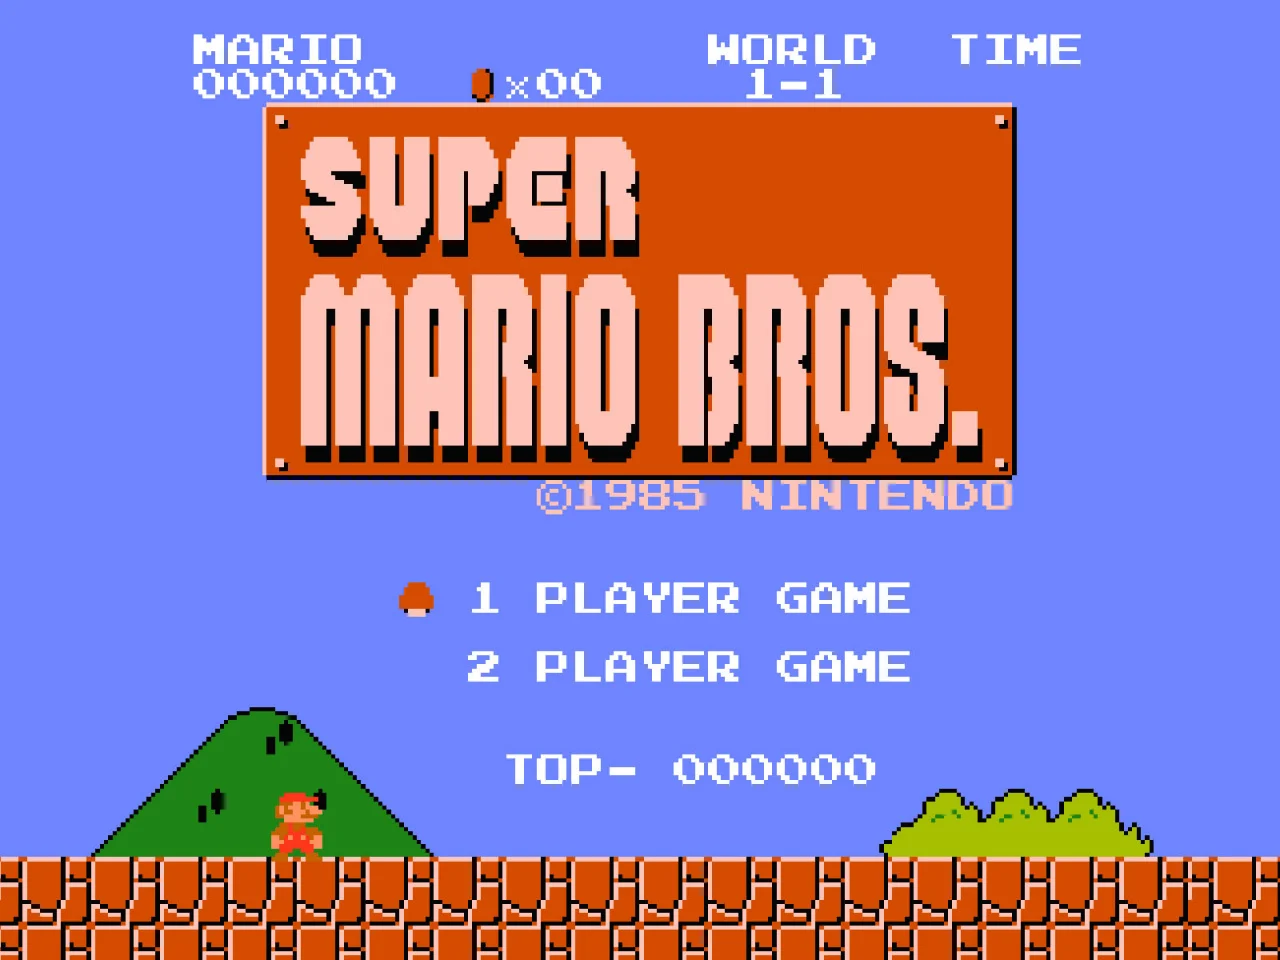
\includegraphics[width=0.8\textwidth]{assets/super-mario-bros.jpg}
    \caption{Super Mario Bros game}
\end{figure}

So this time, I want you to implement some functions about TAS edit action. For your convenient, it is not necessary to test TAS on DS or Wii platform which are require high performance. And your program is required to generate a file named with the extension fm2{\href{https://fceux.com/web/FM2.html}{\tiny link}} for testing on the NES{\href{https://en.wikipedia.org/wiki/Nintendo_Entertainment_System}{\tiny link}} platform, with the classic game being Super Mario Bros. 

There's the description of these function:
\begin{lstlisting}
void button_set_frame(uint8_t **src, size_t *size, const uint8_t button, const uint64_t start_frame, const uint64_t end_frame);
/*
    Parameters: 
        src: Button value array pointer for generate fm2 file.
        size: src size for pointer.
        button: Button uint8_t value to set, not replace.
        start_frame: Represent start frame to set button.
        end_frame: Represent end frame to set button.

    Note:
        If the frame range is overflow, please increase the size of src automatically

    Examples:
        Set 80 value (L, U button) from frame 3 to frame 480.
        
        $ button_set_frame(src, size, 80, 3, 480);
        
        Button set list: R, L, D, U, T, S, B, A. 
        That is uint8_t range value convert to. For example:
               
              RLDUTSBA 
        80 -> 01010000 -> set L, U

        Orginal src:
            {0, 8, 130, 0, 130, 130, 255}
            size of array: 7
            
        After passing the function of src will be:
            {0, 8, 130, 80, 210, 210, 255, 80 ..... 80}
            size of array: 481
*/

void button_unset_frame(uint8_t *src, const size_t size, const uint8_t button, const uint64_t start_frame, const uint64_t end_frame);
/*
    Parameters: 
        src: Button value array for generate fm2 file.
        size: src size for pointer.
        button: Button uint8_t value to unset.
        start_frame: Represent start frame to unset button.
        end_frame: Represent end frame to unset button.

    Examples:
        Unset 2 value (B button) from frame 1 to frame 100.
        
        $ button_unset_frame(src, size, 2, 1, 100);
               
             RLDUTSBA 
        2 -> 00000010 -> unset B

        Orginal src:
            {0, 8, 130, 0, 130, 130, 255}
            size of array: 7
            
        After passing the function of src will be: 
            {0, 8, 128, 0, 128, 128, 253}
            size of array: 7
*/
\end{lstlisting}

TAS achieves high-precision control by manipulating button events frame by frame in a game. To let a NES emulator to do the TAS, the input is provided in the form of an fm2 text file. Each line in the fm2 file represents a button set, as the TAS input for each frame. There's fm2 file example here:

\begin{lstlisting}
|0|........|||  # Frame 0:  Nothing, value: 0
|0|....T...|||  # Frame 1:  Button T event, value: 8
|0|........|||  # Frame 2:  Nothing, value: 0
|0|........|||  # Frame 3:  Nothing, value: 0
|0|R.....B.|||  # Frame 4:  Button R, B event, value: 130
|0|R.....B.|||  # Frame 5:  Button R, B event, value: 130
|0|........|||  # Frame 6:  Nothing, value: 0
|0|........|||  # Frame 7:  Nothing, value: 0
|0|R......A|||  # Frame 8:  Button R, A event, value: 129
|0|R.....B.|||  # Frame 9:  Button R, B event, value: 130
|0|..D.....|||  # Frame 10: Button D event, value: 32
|0|..D.....|||  # Frame 11: Button D event, value: 32
|0|R.....BA|||  # Frame 12: Button R, B, A event, value: 131
|0|RLDUTSBA|||  # Frame 13: All buttons event, value: 255
\end{lstlisting}

The src array to generate fm2 file above is:
\begin{lstlisting}
src: {0, 8, 0, 0, 130, 130, 0, 0, 129, 130, 32, 32, 131, 255}
\end{lstlisting}

To generate fm2 file, I'll give you {\color{red}decode.c} and {\color{red}decode.h} to extract your fm2 file. {\color{red}Please link decode file in Makefile.} The prototype  of function is:
\begin{lstlisting}
void extract_fm2_file(const uint8_t *src, const size_t size);
\end{lstlisting}

I'll use a NES emulator called FCEUX{\href{https://fceux.com/web/home.html}{\tiny link}} while running your fm2 file. To install it, you can run the following command:
\begin{lstlisting}
$ sudo apt install fceux #Ubuntu, Debian
$ sudo brew install fceux #macOS

# Windows version following this URL:
# https://fceux.com/web/download.html

# Note: Maybe other Linux distribution also has repository that able to install FCEUX. You can try to find out yourself.
\end{lstlisting}

Emulator require an NES ROM to start. You can find your ROM {\href{https://github.com/seven7bits/7bits/blob/master/app/roms/Super%20Mario%20Bros.%20(JU)%20(PRG0)%20%5B!%5D.nes}{here}}. And this is how to run it:

\begin{lstlisting}
$ fceux --playmov <your fm2 file> <your NES game ROM>
\end{lstlisting}

There are some FCEUX shortcuts:

\begin{itemize}
\item 
{
NES Gamepad{{\color{blue}\tiny Fig5.4}}  (keyboard map to gamepad button):
    \begin{itemize}
    \item 
    {
    D: B
    }
    \item 
    {
    F: A
    }
    \item 
    {
    Enter: T (Start)
    }
    \item 
    {
    S : S (Select)
    }
    \item 
    {
    Keypad up: U (Up)
    }
    \item 
    {
    Keypad left: L (Left)
    }
    \item 
    {
    Keypad down: D (Down)
    }
    \item 
    {
    Keypad right: R (Right)
    }
    \end{itemize}
}
\item 
{
Show Frame Count: .
}
\item 
{
Frame Speed Up: +
}
\item 
{
Frame Speed Down: -
}
\item 
{
Enter or Quit Fullscreen: 
    \begin{itemize}
    \item 
    {
         Alt + Enter (For Ubuntu or Windows)
    }
    \item 
    {
         Option + Enter (For macOS)
    }
    \end{itemize}
}
\end{itemize}

\begin{figure}[h]
    \centering
    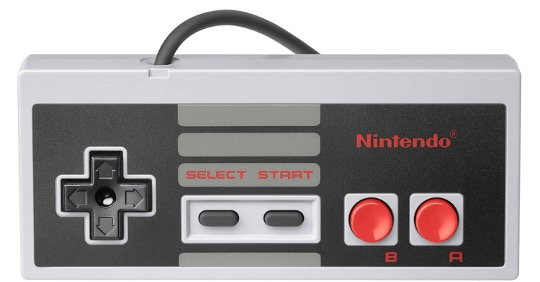
\includegraphics[width=0.8\textwidth]{assets/NES-gamepad.jpg}
    \caption{NES Gamepad}
\end{figure}

You should also prepare a header file called {\color{red}tas.h}. TA will prepare hw0505.c which includes tas.h and uses these functions. {\textbf{\textcolor{blue}{Do not forget to make hw0505.c and decode.c to hw0505 in your Makefile.}}}

\end{document}